\chapter{快速上手}

\LaTeX{}很强大,但对于初学者来说,你不必关心它有多强大,因为最为常用的命令和环境不过寥寥数
个而已。而且Emacs+\auctex{}提供了丰富的快捷键,稍加练习之后,你就再也不用去手工敲命令了。
对于格式复杂的需求,通常你只要套用模版就可以解决问题了。所以,大家只要把Emacs用熟,
一切迎刃而解。

\section{用LaTeX写文章就是在编程}
\label{sec:hello}

\subsection{\texttt{hello.c}}
\label{sec:hello.c}

我们先回忆一下用Emacs写一个\texttt{hello.c}的键盘操作过程:

\begin{enumerate}
\item \Se{},如果你的系统配置和我的一样,那么只要按下\Se{}键,Emacs窗口就
  出现在你面前了,而且(感谢Sawfish)是全屏的;
\item \Cx\Cf{},开始编辑一个新文件。这时,在Emacs窗口的最下面(也就是 mini buffer 里)有提
  示,输入你要编辑的文件的名字,也就是\texttt{hello.c},然后按\Enter{}(回车键),或者\Cj{},其
  实,后面你会发现,\Cj{}带自动缩进,比按\Enter{}更方便;
\item 现在可以在打开的空文件里写东西了:
  \begin{codeblock}[.7]
\begin{ccode}
    #include <stdio.h>
    int main()
    {
      printf ("Hello, world!\n");
      return 0;
    }
\end{ccode}
  \end{codeblock}
\item 存盘:\Cx{}\Cs{}
\item 编译:\texttt{gcc hello.c}
\item 运行:\texttt{./a.out}
\end{enumerate}

\subsection{\texttt{hello.tex}}
\label{sec:hello.tex}

现在,我们再看看用\LaTeX{}写一个\texttt{hello.tex}文件的过程:

\begin{enumerate}
\item \Se{},打开Emacs;
\item \Cx{}\Cf{},\texttt{hello.tex},开始编辑;
\item 写入文件内容:
  \begin{codeblock}[.7]
    \begin{latexcode}
      \documentclass{article}
      \begin{document}
        Hello, world!
      \end{document}
    \end{latexcode}
  \end{codeblock}
\item 存盘:\Cx \Cs{}
\item 编译:\texttt{xelatex hello.tex}
\item 看结果:\texttt{xpdf hello.pdf}
\end{enumerate}

怎么样? \texttt{hello.c}和\texttt{hello.tex}的编辑过程没什么分别吧。只要把Emacs用熟,触
类旁通,不管写什么程序,都是这么个过程。你

\begin{itemize}
\item 不必学习VC去写C/C++;
\item 不必学习eclipse去写Java;
\item 不必学习MS-Word去写报告、幻灯片;
\item 不必学习……
\end{itemize}

一句话,“Everything Emacs”,你可以省下大量不必要的学习时间。人生苦短,何必让你的生活
被 VC/eclipse/MS-Word 搞得头昏脑胀呢? 简单而强大,就是计科专业和非专业学生所应有的不同。

如果你对Emacs操作还很陌生,那么现在就打开Emacs,\Ch{}{\kbd t},重温一下那些基本操
作吧。

\subsection{什么是 \Cx\Cf?}

使用Emacs是可以(而且应该)完全抛开鼠标的。对于初次上手的人,抛开鼠标就像病人抛开拐杖一
样痛苦。但只有不依赖拐杖的人才是健康的,不是吗?

现在,你终于有了走向健康生活的冲动,那么我们开始吧。简短截说,

\begin{enumerate}
\item 先把你的双手在标准键盘上放好。然后,
\item 左手小指稍向左移,按在\Caps{}(CapsLock)键上\footnote{如果你的系统配置和我一
    样,那么\Caps{}就是\Ctrl{}键。},按住别放开,
\item 左手无名指稍向下移,在{\kbd x}键上轻按一下就放开,这就是\Cx{};
\item 小指按在\Caps{}上别放开,左手食指在{\kbd f}键上轻按一下就放开,这就是\Cf{};
\item 现在左手小指可以放开了。
\end{enumerate}

这就是\Cx\Cf{},最常用的Emacs快捷键之一,作用是要求打开一个文
件\footnote{如果你要打开的文件不存在,那么Emacs会认为你要写一个新文件。},f代表file 。那么,
告诉我

\begin{itemize}
\item 什么是 \Cx \Cs?
\item 什么是 \Cx {\kbd 2}? 什么是\Cx {\kbd 3}? 什么是\Cx {\kbd o}? 什么是\Cx {\kbd 0}? 什么
  是\Cx {\kbd 1}?
\item 什么是\Cx {\kbd h}? 什么是\Cw{}?
\item 什么是 \Cg{}?
\item 什么是\Cj{}? 什么是 \Ci{}?
  % \item 什么是 \LKeyCtrlX{/}?
\item 什么是 \Ck{}? 什么是 \Cy{}?
\item 什么是\Cd{}? 什么是 \Cd{}?% (M 代表 Meta 键, 也就是 Alt 键)
\item 什么是 \Ca{}? 什么是\Ce{}? 什么是\Cf{}? 什么是\Cb{}?
  什么是\Cn{}? 什么是\Cp{}?
\end{itemize}

如果你还不熟悉上面这些快捷键,那么用起Emacs来,就会像西洋人用筷子一样不酷。(「嘿!把你的手从
鼠标上拿开!」)刚甩开拐杖,走向健康生活的人,总会不自觉地去扶点什么,这很正常。但你一定要坚
持锻炼,不要让这种「正常」持续得太久。今后的生活能否轻松愉快,主要就取决于你的「健康」程度。
如果有朝一日你真的抛开了鼠标,那么即使面对一个纯字符界面的终端,你也能写出漂亮的PDF格式的论
文。作为计科专业的学生,好歹该比网吧青年们酷一些嘛。

\section{生活可以更轻松}

\auctex{}是Emacs的一个功能模块,为\LaTeX{}编程提供了巨大的便利。有了它,你的\LaTeX{}生活可以
像 \texttt{Hello, world!}一样简单。现在就跟着我,手把手地领略一下简单的乐趣吧。

一切当然是从\Se{},打开Emacs开始。然后,\Cx\Cf{},让我们开
始编辑一个新文件,就叫 \texttt{simple.tex}吧。

在Emacs窗口的最下方,也就是 mini buffer 里,这时应该会有提示,让你输入文件名。输
入\texttt{simple.tex}, 然后按 \Cj{}。如果这时 mini buffer 里有如下提示:

\begin{itemize}
\item[] \texttt{Master file: (default this file) ...}
\end{itemize}

直接按 \Cj{} 就可以了。知道了吧, \Cj{} 就是我们的\Enter{}(回车)键。如果你的手正放在「标准
键盘」上,那么,左手小指向左一偏,按到的正是\Ctrl{}键(\Caps{}{\scriptsize (CapsLock)}被我
们改造成\Ctrl{}了)。右手食指下不正是{\kbd j}键吗?怎么样,比\Enter{}更方便吧。

现在,可以向 \texttt{simple.tex}文件里写东西了,\Cc\Ce{},e代表environment。“环境”到底是什么
呢?意会吧,用用就明白了。在 mini buffer 里会有提示,

\begin{itemize}
\item[] \texttt{Environment type: (default document)}
\end{itemize}

这是在问你是不是要写一篇document(文章)啊?你当然该用\Cj{}来告诉它「是」。这时,mini buffer 又会提示,

\begin{itemize}
\item[] \texttt{Document class: (default article)}
\end{itemize}

这是在问你是不是要写一篇 article 类型的文章啊?除了 article,通常还有 book, report, letter
可供选择。我们现在碰巧就是要写个短小的 article,所以,按\Cj{}确认就好。这时, mini buffer 继续提示,

\begin{itemize}
\item[] \texttt{Options:}
\end{itemize}

这是在问你是否有什么特殊选项啊?用\Cj{}来告诉它说「不需要」。现在,你的 \texttt{simple.tex}
文件里应该有如下几行东西了:
\begin{codeblock}[.9]
\begin{latexcode}
  \documentclass{article}  % documentclass可以是
                           % article, book, report, letter...
  \begin{document} % 文章的开始
  | 
  \end{document}   % 文章的结束
\end{latexcode}
\end{codeblock}
这时,光标停在 \verb|\begin{document}|与 \verb|\end{document}|之间,等待你的输入。百分号
(\verb|%|)后面显然都是注释。

在第\ref{sec:hello}节里,你已经会写 \texttt{Hello, world!}了。现在,我们要写点像模像样的东
西。偷懒起见,我直接\xpinyin{套}{chao1}\xpinyin{用}{xi2}Andrew Roberts 写的%
\texttt{simple.tex}\footnote{\url{http://en.wikibooks.org/wiki/LaTeX/simple.tex}}。我们把注
意力集中在用Emacs写文章的过程上。

\subsection{Top matter}

先确保你的光标在 \verb|\begin{document}| 和 \verb|\end{document}| 之间,也就是文章的
第4行。然后按\Cc \Cm{},这时 mini buffer 里会有如下提示:

\begin{itemize}
\item[] \verb|Macro (default ref): \|
\end{itemize}

这是系统在等待你输入一个 \texttt{Macro},说白了就是“命令”。输入:\texttt{title},\Cj{},这时
你的文章会变成下面这样:

\begin{codeblock}[.9]
\begin{latexcode}
  \documentclass{article}  % documentclass可以是
                           % article, book, report, letter...
  \begin{document}         % 文章的开始
  \title{|} 
  \end{document}           % 文章的结束
\end{latexcode}
\end{codeblock}

这时,光标停在 \verb|\title{}| 的花括号里。不用说你也知道,该输入文章的标题了。那么就给它
一个标题:

\begin{codeblock}[.9]
\begin{latexcode}
  \documentclass{article}  % documentclass可以是
                           % article, book, report, letter...
  \begin{document} % 文章的开始
  \title{How to Structure a \LaTeX{} Document} 
  \end{document}   % 文章的结束
\end{latexcode}
\end{codeblock}
发现了吗?凡是以反斜杠开头的都是命令(\texttt{Macro}), 比如 \verb|\LaTeX{}|,它的唯一作用
就是把 \texttt{LaTeX} 这五个字母输出成一副怪样子,\LaTeX{}。

好了,在 title 下新起一行。然后\Cm{}。你肯定知道 \Cm{}是干什么用的了吧,就是要输入一
个 Macro。也许你会好奇,想知道总共有多少 Macro? 那么现在可以按一下{\Tab}键。看到了吗?在弹
出的新窗口中,列出了近百个 Macro. 还好,我们并不需要记住这么多。最常用的也就三、五个而已。

mini buffer 里又会有提示:

\begin{itemize}
\item[] \verb|Macro (default title): \|
\end{itemize}

Emacs会把我们上次输入的Macro,也就是title,做为默认值提示出来。不用管它,输入:
\texttt{author} \Cj{}。然后在 \verb|\author{}| 的花括号里输入作者的名字。当然,也可以把自己
的通信地址、email写在里面。就像下面这样:
\begin{codeblock}[.9]
\begin{latexcode}
  \documentclass{article}  % documentclass可以是
                           % article, book, report, letter...
  \begin{document}         % 文章的开始
  \title{How to Structure a \LaTeX{} Document}
  \author{Andrew Roberts\\
    School of Computing,\\
    University of Leeds,\\
    Leeds,\\
    United Kingdom,\\
    LS2 1HE\\
    \emph{andyr@comp.leeds.ac.uk}}
  \end{document}           % 文章的结束
\end{latexcode}
\end{codeblock}
注意,\verb|\\|代表“强制换行”。现在,新起一行,加上日期:

\begin{enumerate}
\item \Cc\Cm{} date \Cj
\item \Cc\Cm{} today \Cj
\end{enumerate}

其实,如果没有 \verb|\date{\today}| 这一句,系统会自动把今天的日期添加上的。而
且 \verb|\date{}|里面的日期你可以随意写,不一定非要是当天的日期。title, author, date 一般被
叫做文章的 top matter(开头那点事)。

再新起一行,写 \verb|\maketitle| \Cj{}。\verb|\maketitle| 自然是要排版top matter了。换句
话说,不要标题的话可以省略掉这个命令。现在文章变成了这样:
\begin{codeblock}[.9]
\begin{latexcode}
  \documentclass{article}  % documentclass可以是
                           % article, book, report, letter...
  \begin{document}         % 文章的开始
  \title{How to Structure a \LaTeX{} Document}
  \author{Andrew Roberts\\
    School of Computing,\\
    University of Leeds,\\
    Leeds,\\
    United Kingdom,\\
    LS2 1HE\\
    \emph{andyr@comp.leeds.ac.uk}}
  \date{\today}
  \maketitle
  \end{document}           % 文章的结束
\end{latexcode}
\end{codeblock}
好奇的话,现在可以编译一下,看看PDF文件的效果:

\begin{enumerate}
\item 编译:\Cc\Cc\Cj
\item 查看:\Cc\Cv
\end{enumerate}

这时,一个PDF文件应该显示在屏幕上了(图\ref{fig:topmatter})。效果还满意吧?保持你的好奇心。在下面的操作中,你随时可
以编译一下看看效果。

\begin{figure}
  \centering
  \begin{minipage}{.4\linewidth}
  \fbox{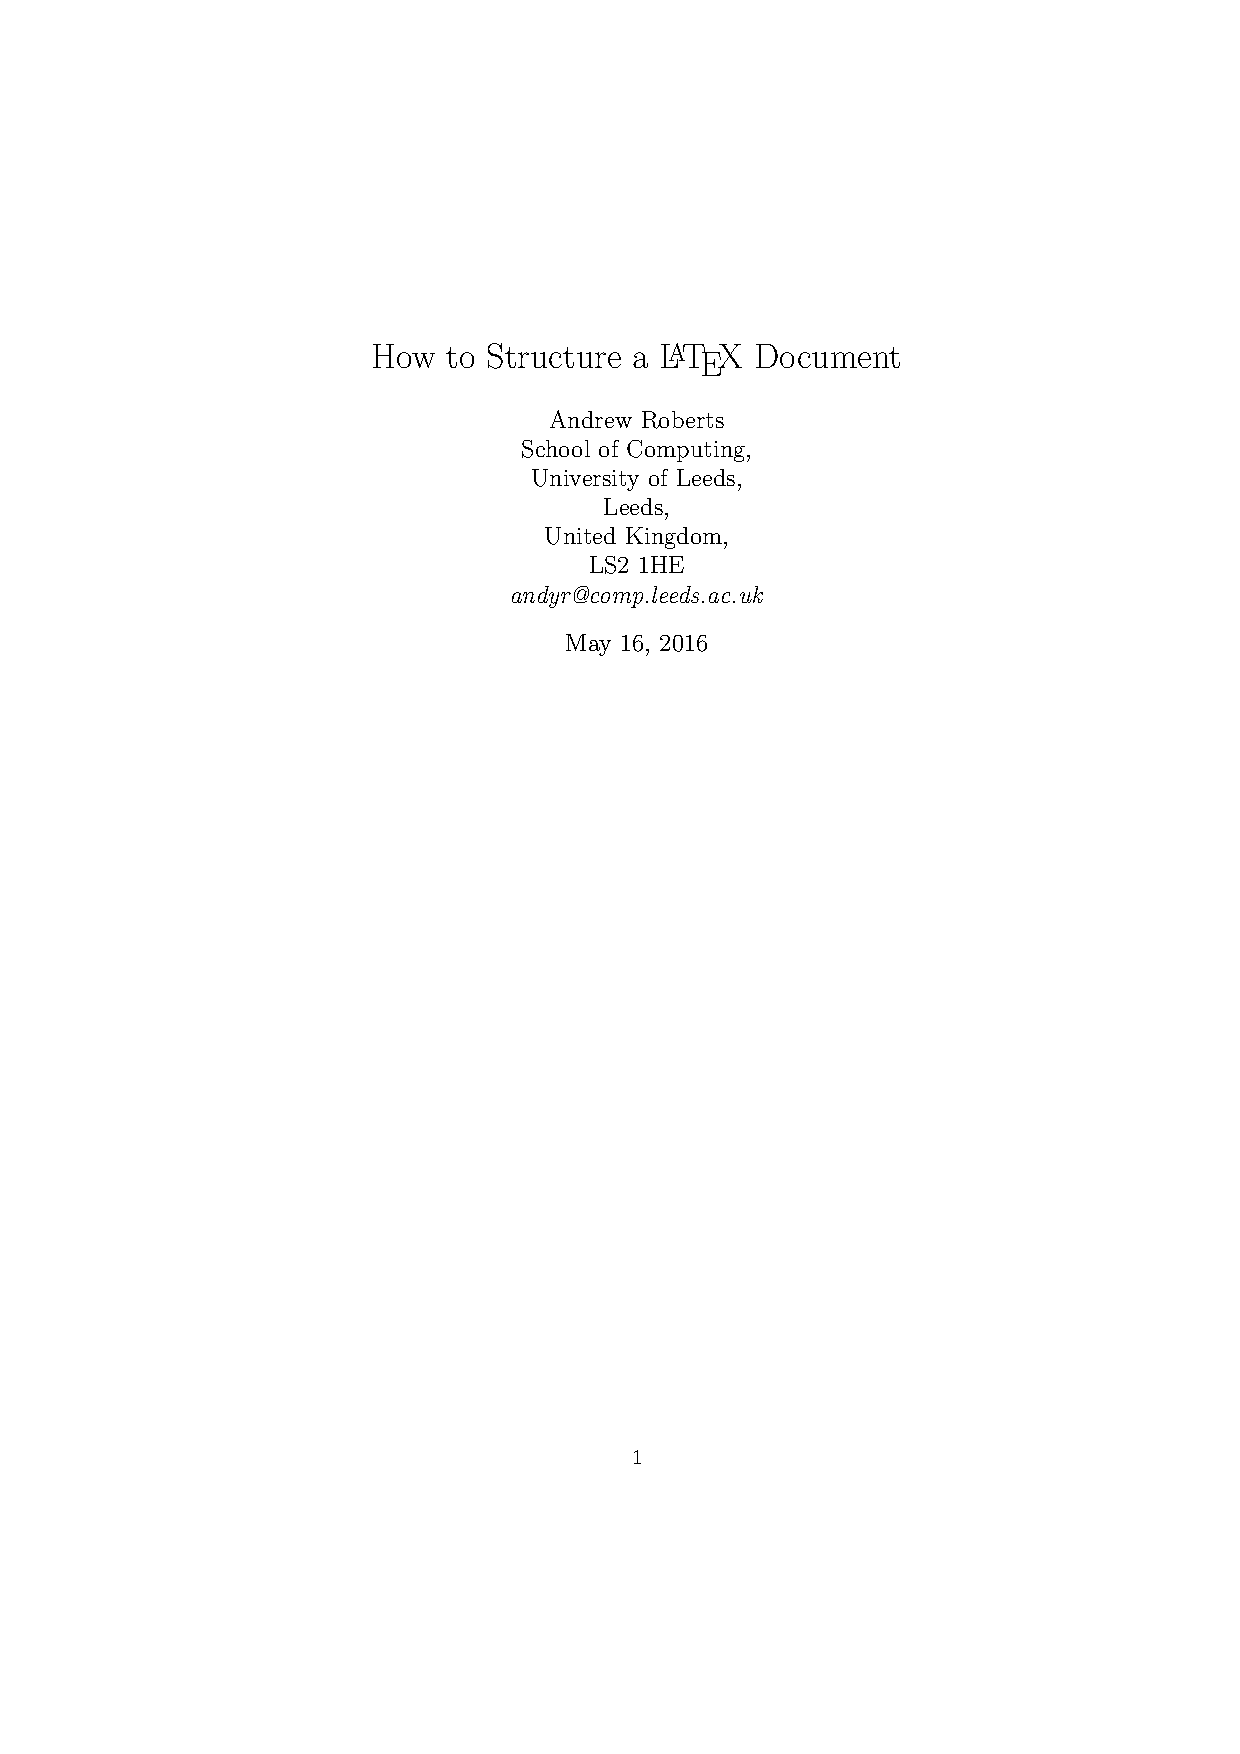
\includegraphics[width=\textwidth]{topmatter}}
  \caption{文章的起始部分} \label{fig:topmatter}
  \end{minipage}\quad
  \begin{minipage}{.4\linewidth}
    \fbox{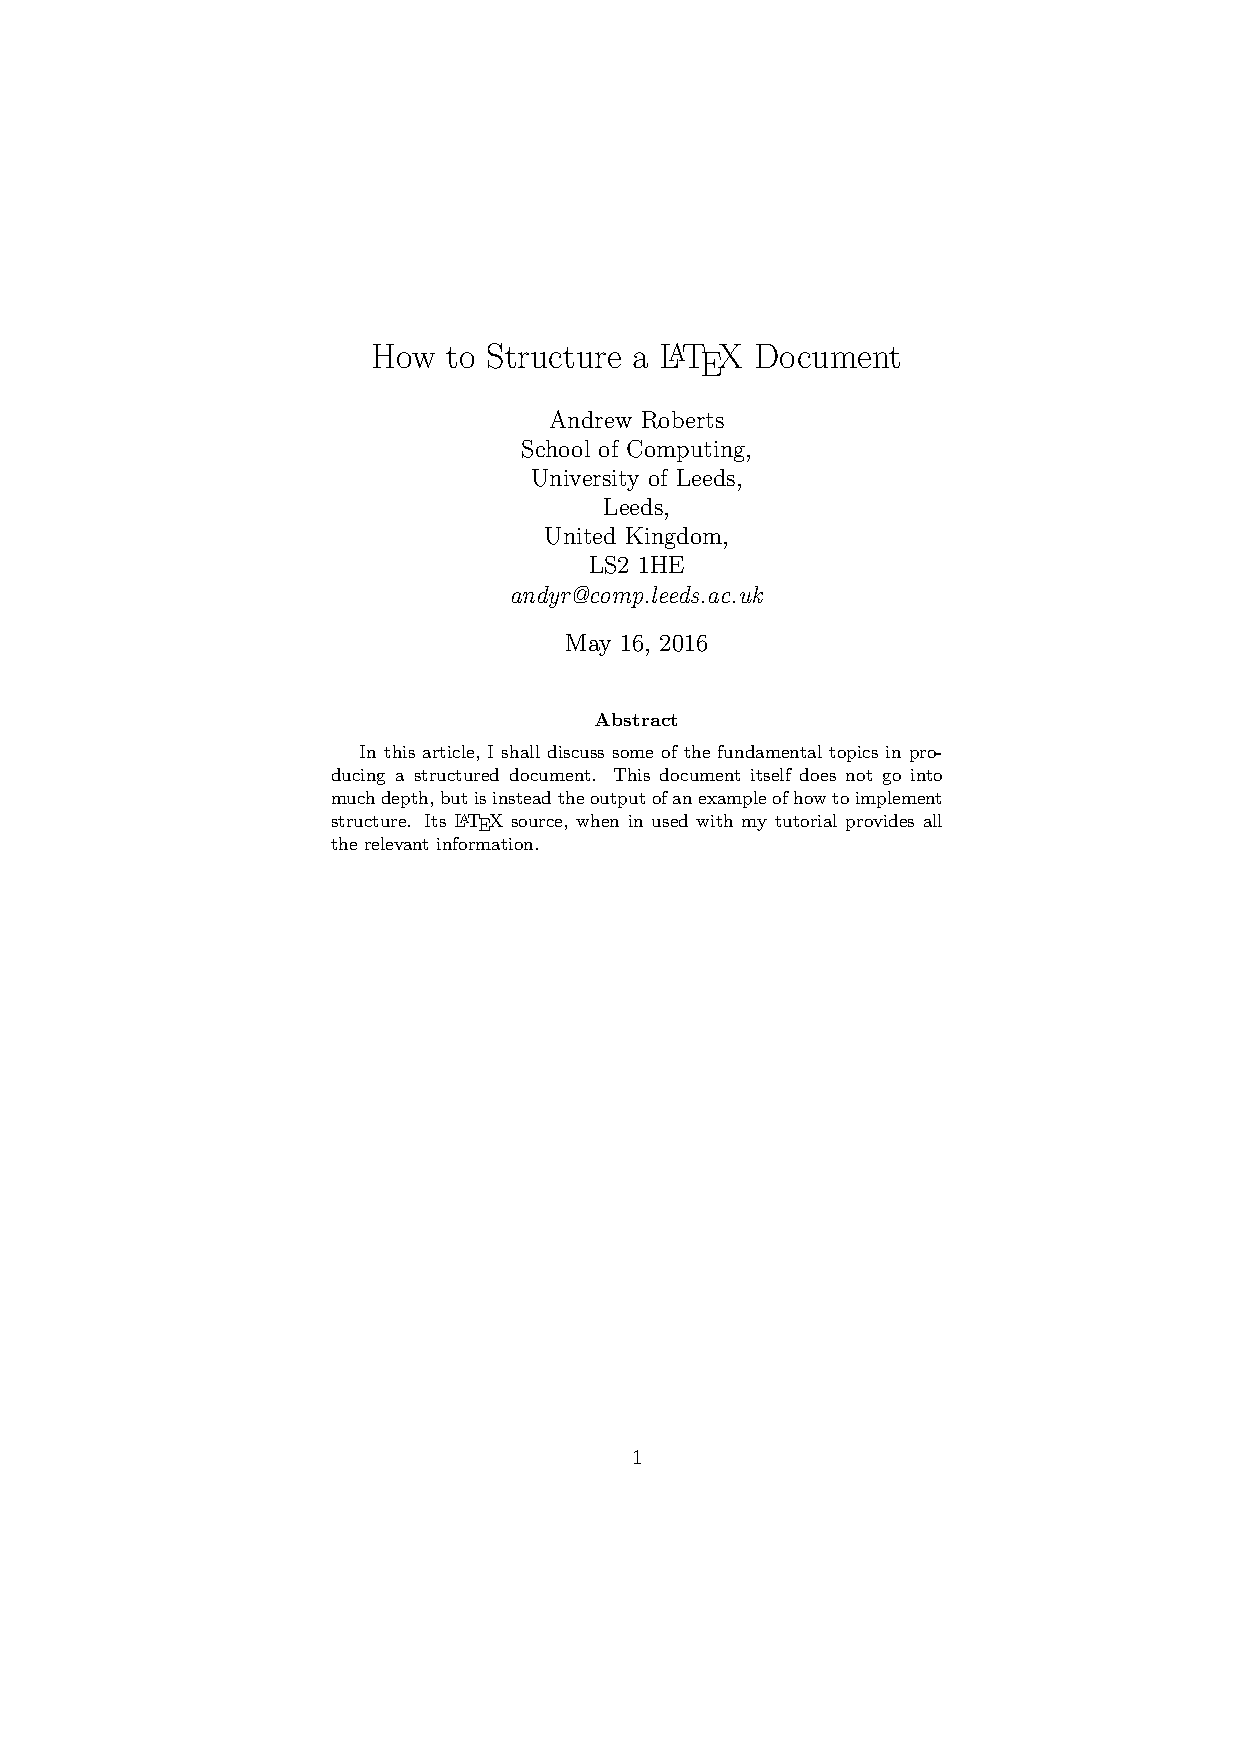
\includegraphics[width=\textwidth]{abstract}}
  \caption{加上摘要} \label{fig:abstract}
  \end{minipage}
\end{figure}

\subsection{怎样写摘要}

好了,回到Emacs。现在你的光标应该停在 \verb|\maketitle| 的下面一行。我们开始写「摘要」部
分。\Cc\Ce{},开始一个新的“环境”\footnote{如果你好奇心强,想知道总共有哪些“环境”的话,现在
  可以按{\Tab}键。}。mini buffer 里提示:

\begin{itemize}
\item[] \texttt{Environment type: (default itemize)}
\end{itemize}

这是在问你要开始哪个环境啊?默认是开始 itemize 环境,因为它是最常用的环境。但我们现在要写的是“摘要”,告诉它:
abstract \Cj{}。abstract 就是“摘要”的意思。科技论文都是要有摘要的嘛。于是,你的文章变成了这样:
\begin{codeblock}[.9]
\begin{latexcode}
  % 此处略去十数行
 
  \maketitle
 
  \begin{abstract} 
    |
  \end{abstract}
  \end{document}           % 文章的结束
\end{latexcode}
\end{codeblock}
光标停在 \verb|\begin{abstract}| 和 \verb|\end{abstract}| 之间(第6行)。好,现在往摘要部分里填点东西:
\begin{codeblock}[.9]
\begin{latexcode}
  % 此处略去十数行
 
  \maketitle
 
  \begin{abstract} 
    In this article, I shall discuss some of the fundamental
    topics in producing a structured document.  This
    document itself does not go into much depth, but is
    instead the output of an example of how to implement
    structure. Its \LaTeX{} source, when in used with
    my tutorial provides all the relevant information.
  \end{abstract}
  \end{document}           % 文章的结束
\end{latexcode}
\end{codeblock}
看看效果(图\ref{fig:abstract})。

\subsection{怎样分章节}

现在,我们要接着上面的例子,写更多更长的东西了。偷懒起见,文章末尾
的 \texttt{\textbackslash{}end\{document\}}我也不再写出来了。

好,按\Cn{}把光标移到 \verb|\end{abstract}| 的下一行。然后,\Cc\Cs{},让我们开始文章的第一节。
s 代表 section, “节”的意思。mini buffer 提示:

\begin{itemize}
\item[] \texttt{Level: (default section) }
\end{itemize}

显然是在问你,要不要起一个新 section 啊?没错,我就是要起一个新的章节,于是直接\Cj{}。
mini buffer 又提示:

\begin{itemize}
\item[] \texttt{Title:}
\end{itemize}

也就是问你,章节标题是……?那就给它个标题吧,就叫“Introduction”。\Cj{}之后, mini buffer 继续提示:

\begin{itemize}
\item[] \texttt{Label: sec:introduction}
\end{itemize}

这是在问你,要不要给这个新章节打个标签,比如 \texttt{sec:introduction}, 以后也许要索引到它呢?
这个暂时无关紧要,\Cj{}就行了。于是,文中又有了下面的第5、6两行。
\begin{codeblock}[.9]
\begin{latexcode}
  % 此处略去十数行

  \end{abstract}

  \section{Introduction}
  \label{sec:introduction}
\end{latexcode}
\end{codeblock}
给这一节添加内容:
\begin{codeblock}[.9]
\begin{latexcode}
  % 此处略去十数行

  \end{abstract}

  \section{Introduction}
  \label{sec:introduction}

  This small document is designed to illustrate how easy
  it is to create a well structured document within
  \LaTeX\cite{lamport94}.  You should quickly be able to
  see how the article looks very professional, despite the
  content being far from academic.  Titles, section
  headings, justified text, text formatting etc., is all
  there, and you would be surprised when you see just how
  little markup was required to get this output.
\end{latexcode}
\end{codeblock}
注意到了吗?在这一节里有一个新命令 \verb|\cite{}|, 这是在引用一个参考文献。先不管它,后面再说。

如法炮制,再添加几个章节:
\begin{longlisting}
\begin{latexcode}
  % 此处略去十数行

  \end{abstract}

  \section{Introduction}
  \label{sec:introduction}

  This small document is designed to illustrate how easy
  it is to create a well structured document within
  \LaTeX\cite{lamport94}.  You should quickly be able to
  see how the article looks very professional, despite the
  content being far from academic.  Titles, section
  headings, justified text, text formatting etc., is all
  there, and you would be surprised when you see just how
  little markup was required to get this output.

  \section{Structure}
  \label{sec:structure}
  
  One of the great advantages of \LaTeX{} is that all it
  needs to know is the structure of a document, and then it
  will take care of the layout and presentation itself. So,
  here we shall begin looking at how exactly you tell
  \LaTeX{} what it needs to know about your document.
  
  \subsection{Top Matter}
  \label{sec:top-matter}
  
  The first thing you normally have is a title of the
  document, as well as information about the author and
  date of publication. In \LaTeX{} terms, this is all
  generally referred to as \emph{top matter}.

  |
\end{latexcode}
\end{longlisting}

注意到 \verb|\emph{}| 了吗?它代表 emphasize ,“强调”。英文习惯用斜体字来表示强调的东西,那
么 \verb|\emph{hello, world}| 自然就是把 hello, world 排版成 \emph{hello, world} 了。

注意到 \verb|\subsection{}| 了吗?一会儿,我们还会看到 \verb|\subsubsection|。不用解释吧,
文章的章节次序是这样:

\begin{minipage}{.6\linewidth}
  \begin{singlespace}
    \begin{multicols}{3}
      \begin{enumerate}
      \item chapter
      \item section
      \item subsection
      \item subsubsection
      \item paragraph
      \item subparagraph
      \end{enumerate}
    \end{multicols}
  \end{singlespace}
\end{minipage}\par\vspace{2ex}

其中的chapter,只有在 book 和 report 中才能使用,而 article 只能用 section 以下的东西。

现在我们就来增加一个 subsubsection。不出所料的话,光标现在应该在第34行。那么
就\Cc\Cs{},mini buffer 提示:

\begin{itemize}
\item[] \texttt{Level: (default subsection)}
\end{itemize}

当然输入:subsubsection \Cj{}。mini buffer 提示:

\begin{itemize}
\item[] Title:
\end{itemize}

输入:Article Information \Cj。mini buffer 提示:

\begin{itemize}
\item[] \texttt{Label: sec:article-information}
\end{itemize}

似曾相识吧?敲\Cj{},于是,文章中又有了如下两行:
\begin{codeblock}[.9]
\begin{latexcode}
  \subsubsection{Article Information}
  \label{sec:article-information}
\end{latexcode}
\end{codeblock}
也就是说,我们有了一个 subsubsection。

\subsection{什么是环境}

现在,我们来添加一个 environment。\Cc\Ce{},mini buffer 提示:

\begin{itemize}
\item[] \texttt{Environment type: (default abstract)}
\end{itemize}

我们当然不再需要 abstract 了,现在我们要的是 itemize ,也就是“不带序号的列表”。那么当然输
入:itemize \Cj{}。于是看到:
\begin{codeblock}[.9]
\begin{latexcode}
  \begin{itemize}
  \item |
  \end{itemize}
\end{latexcode}
\end{codeblock}
光标停在 \verb|\item| 的后面。非常好,这正是我想要的。于是直接输入如下文字:

\begin{itemize}
\item[] \verb'\verb|\title{}| --- The title of the article.'
\end{itemize}

输入之后,\MEnter{},也就是,左手拇指按住{\kbd }键,同时右手小指去敲\Enter{}。你会看到
这样的效果:
\begin{codeblock}[.9]
\begin{latexcode}
  \begin{itemize}
  \item \verb|\title{}| --- The title of the article.
  \item 
  \end{itemize}
\end{latexcode}
\end{codeblock}
也就是说,不仅换了行,而且自动有了 \verb|\item|等待你输入新的东西。

你一定注意到了 \verb'\verb||' 这个新命令。它的作用和bash命令行的单引号 (\texttt{'}) 是一样的。
还记得吧,在命令行,单引号里的东西是原样输出的。 \verb'\verb||' 里的东西也一样。 verb 是
verbatim 一词的缩写,就是“原样引用”的意思。好奇的话,可以编译一下,看看效果。

\begin{center}
  \fbox{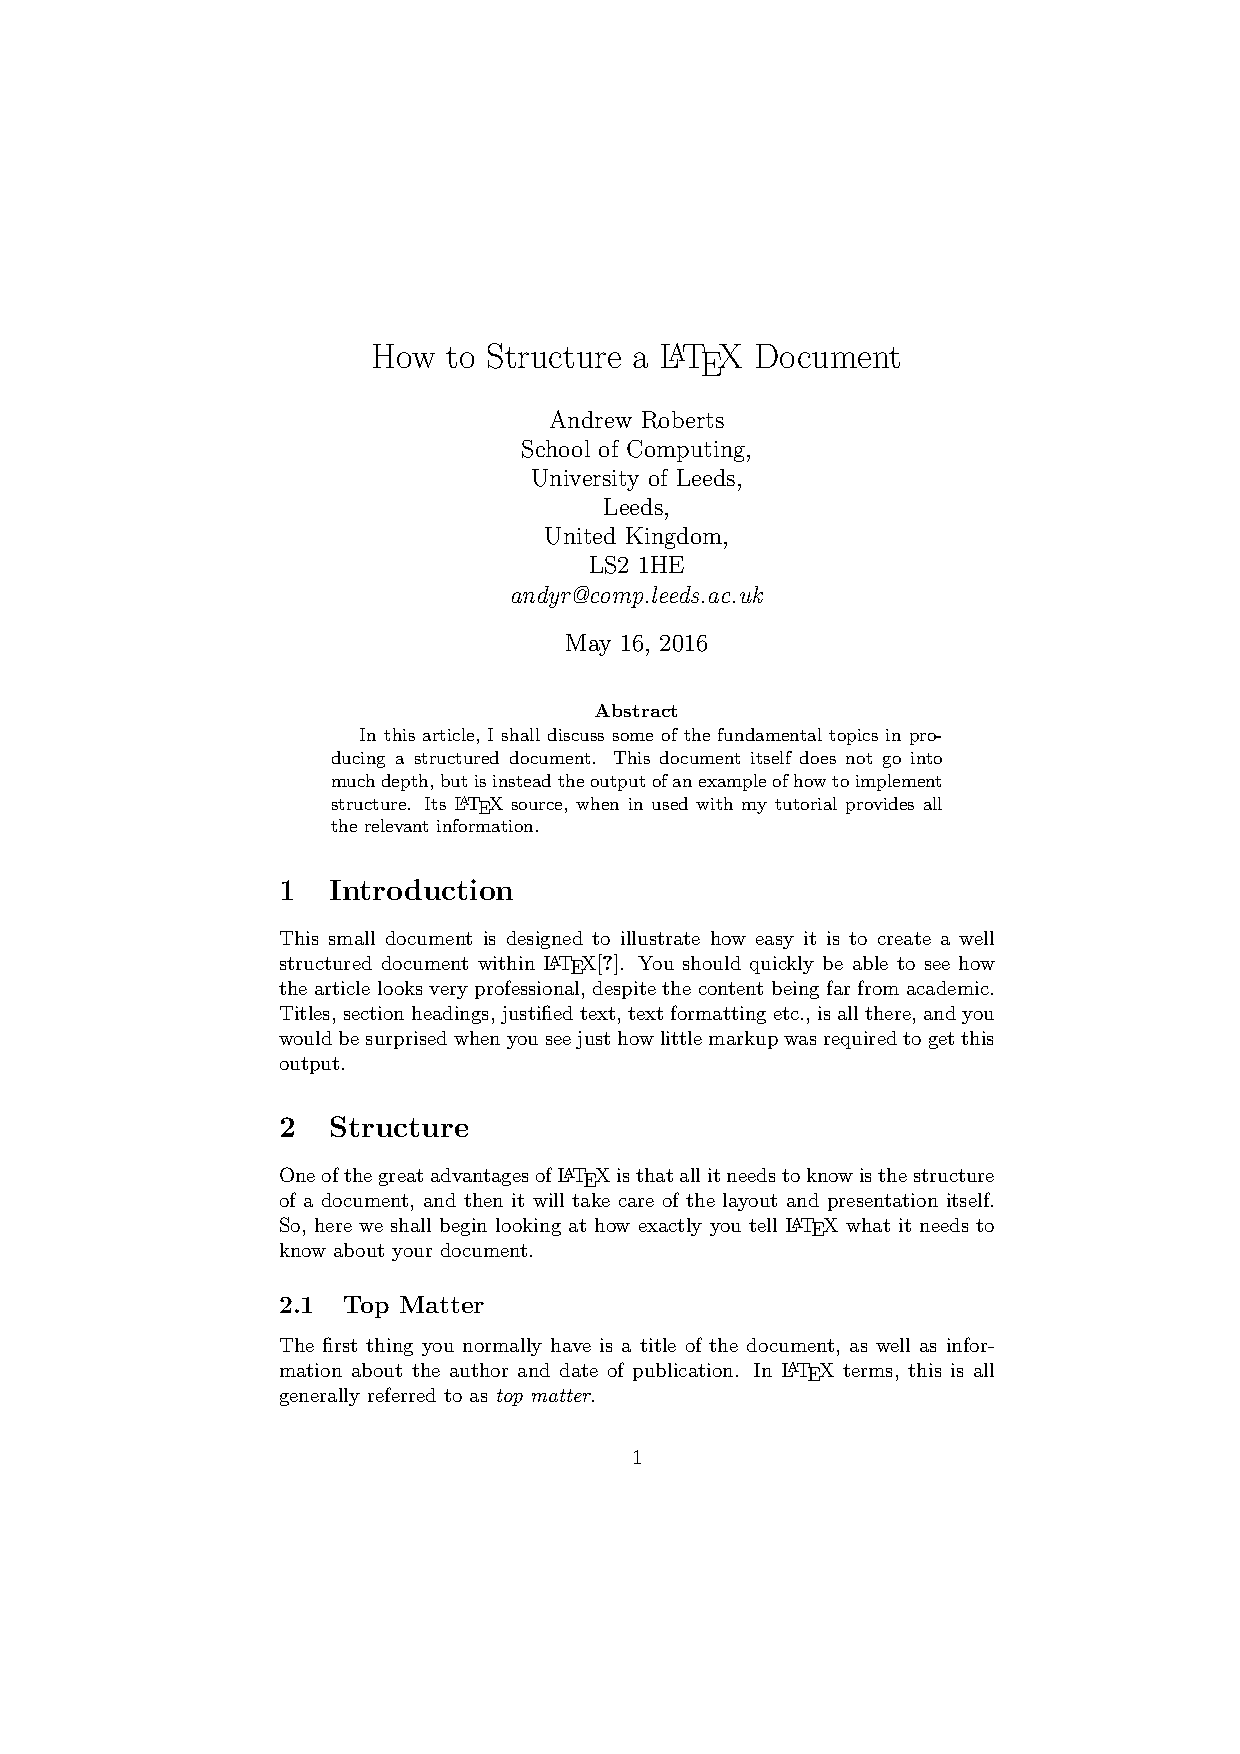
\includegraphics[width=.48\textwidth]{env1}}
  \fbox{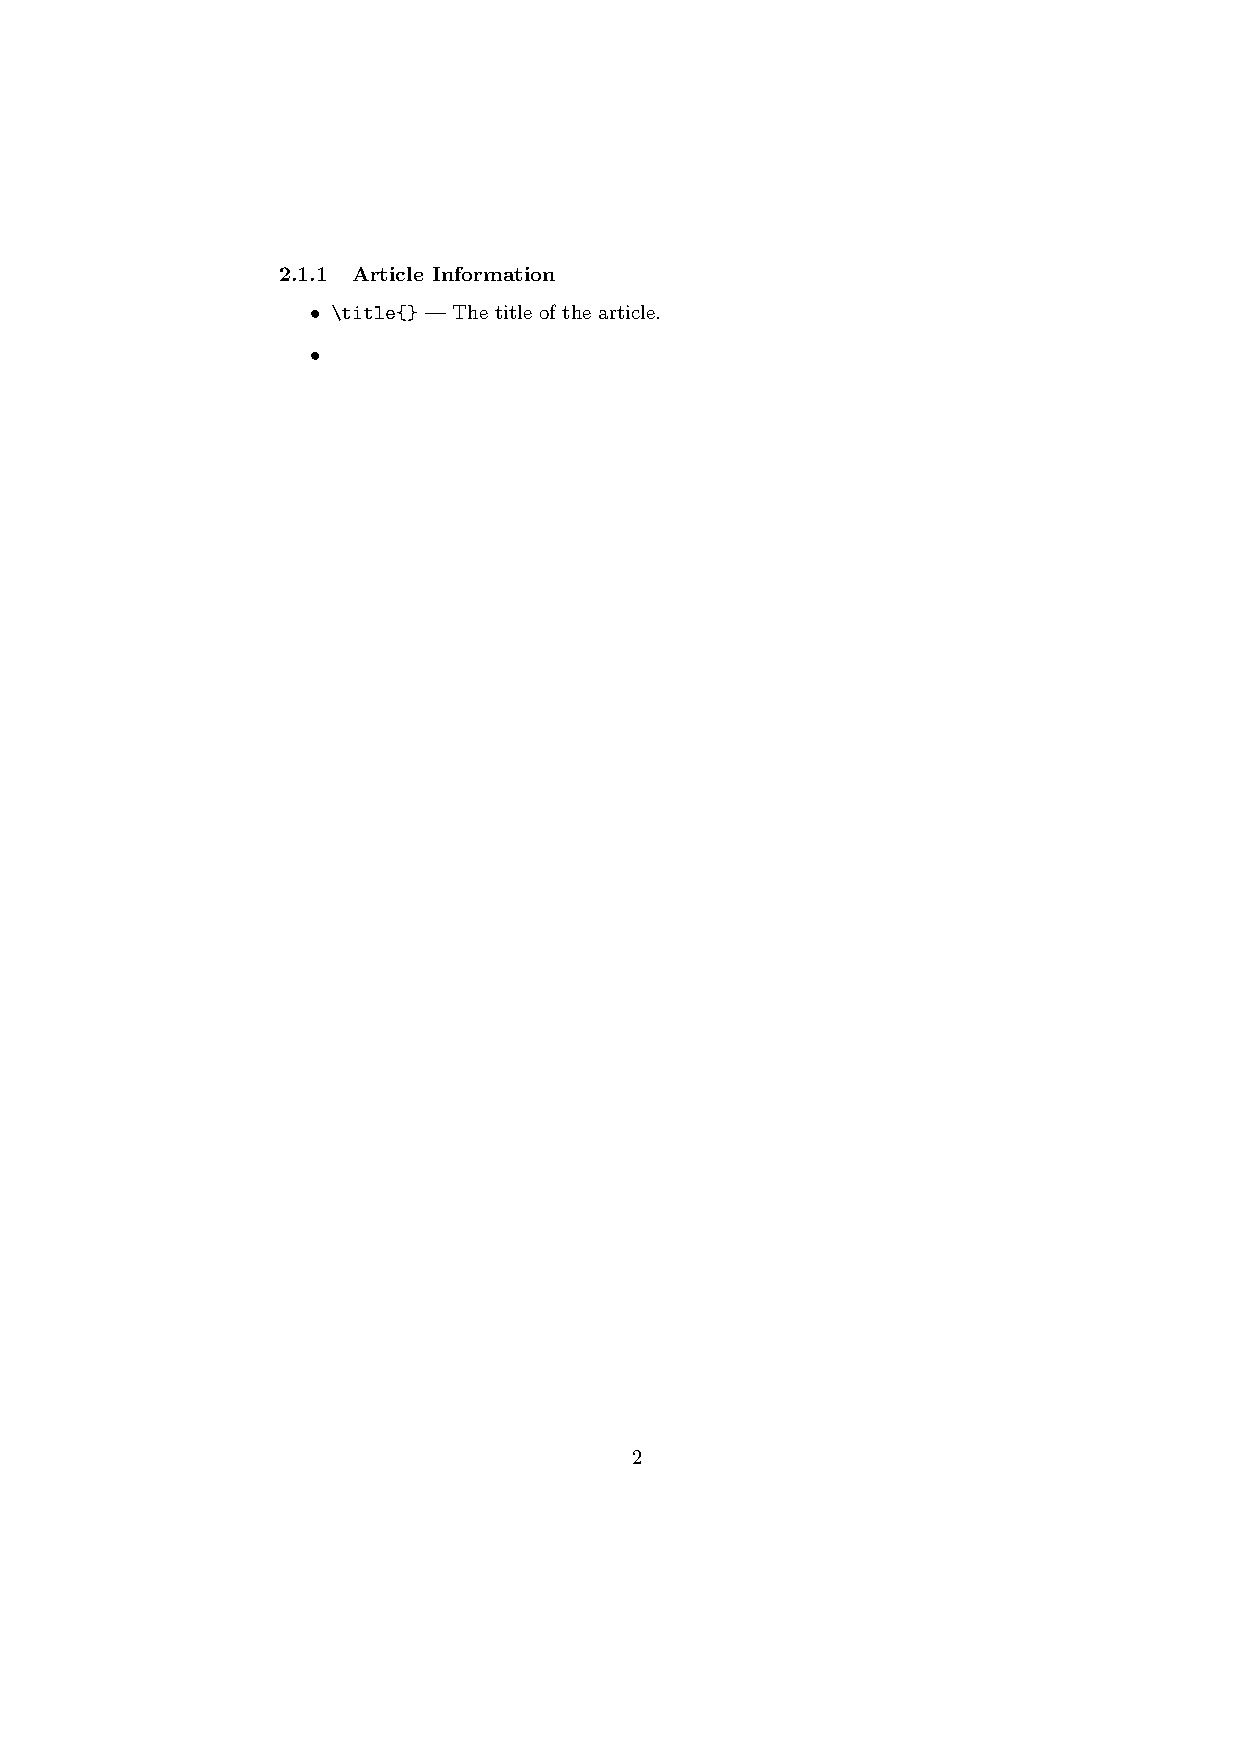
\includegraphics[width=.48\textwidth]{env2}}
\end{center}

好,继续输入:

\begin{itemize}
\item[] \verb'\verb|\date| --- The date. Use:'
\end{itemize}

得到:
\begin{codeblock}[.9]
\begin{latexcode}
  \begin{itemize}
  \item \verb|\title{}| --- The title of the article.
  \item \verb|\date| --- The date. Use: 
  \end{itemize}
\end{latexcode}
\end{codeblock}
没什么好说的。现在我们要在 itemize 环境里面再套一个 itemize 。光标现在应该在第3行的最后。
敲:\Cc\Ce\Cj{},于是得到:

\begin{codeblock}[.9]
\begin{latexcode}
  \begin{itemize}
  \item \verb|\title{}| --- The title of the article.
  \item \verb|\date| --- The date. Use:
    \begin{itemize}
    \item 
    \end{itemize}

  \end{itemize}
\end{latexcode}
\end{codeblock}

简单吧?不用说了,你肯定知道下面这些是怎么来的了吧。

\begin{codeblock}[.9]
\begin{latexcode}
  \begin{itemize}
  \item \verb|\title{}| --- The title of the article.
  \item \verb|\date| --- The date. Use:
    \begin{itemize}
    \item \verb|\date{\today}| --- to get the date that
      the document is typeset.
    \item \verb|\date{}| --- for no date.
    \end{itemize}
  \end{itemize}
\end{latexcode}
\end{codeblock}

编译之后的效果应该和下面这张图差不多。

\begin{center}
  \fbox{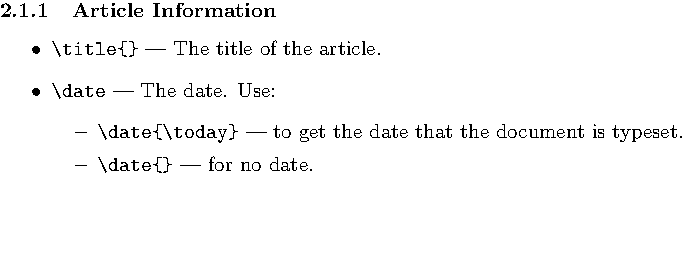
\includegraphics[width=.5\textwidth]{env3-crop}}
\end{center}

好了,请你现在照猫画虎,再来一个 subsubsection,标题叫 Author Information。模仿上面的东西,
来得到下面的东西:

\begin{codeblock}[.9]
\begin{latexcode}
  \subsubsection{Author Information}
  \label{sec:author-information}
  
  The basic article class only provides the one command:
  \begin{itemize}
  \item \verb|\author{}| --- The author of the document.
  \end{itemize}
  
  It is common to not only include the author name, but
  to insert new lines (\verb|\\|) after and add things
  such as address and email details.  For a slightly more
  logical approach, use the AMS article class (\emph{amsart})
  and you have the following extra commands:
  
  \begin{itemize}
  \item \texttt{address} --- The author's address.  Use the
    new line command (\verb|\\|) for line breaks.
  \item \texttt{thanks} --- Where you put any acknowledgments.
  \item \texttt{email} --- The author's email address.
  \item \texttt{urladdr} --- The URL for the author's web page.
  \end{itemize}
\end{latexcode}
\end{codeblock}

显示效果:

\begin{center}
  \fbox{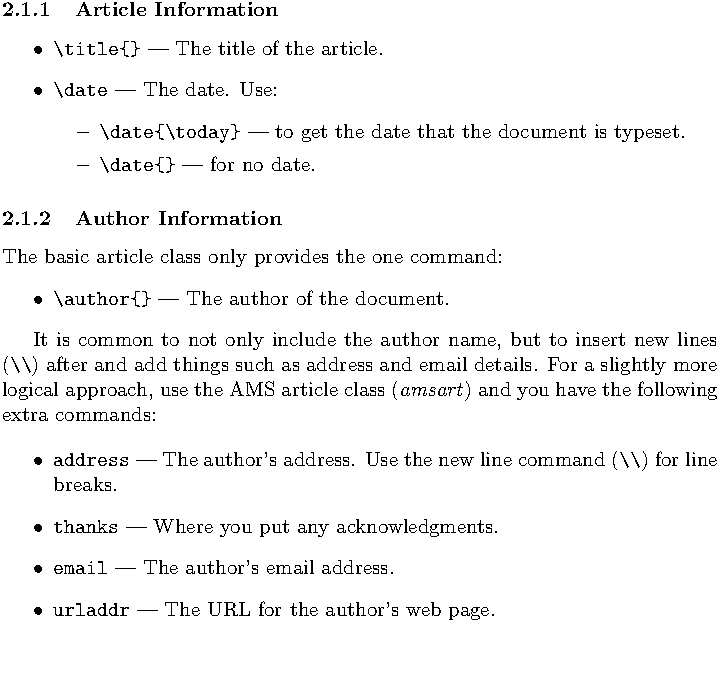
\includegraphics[width=.6\textwidth]{env4}}
\end{center}

怎么样,不太困难吧? 目前为止,我们用到的无非是表~\ref{tab:keys}中列出的这几个快捷键操作
而已:

\begin{table}[!htbp]
  \centering
  \caption{常用快捷键}\label{tab:keys}
  \begin{tabu*}to .5\textwidth {X[r,-1]|X[l,-1]}
    \hline
    \rowfont[c]{\bfseries}快捷键&功用\\\hline
    \Cj{}&换行带缩进\\
     \Cc\Cm{}&输入Macro\\
     \Cc\Cs{}&新起一个章节\\
     \Cc\Ce{}&新起一个环境\\
     \MEnter{}&换行带 \textbackslash\texttt{item}\\\hline
  \end{tabu*}
\end{table}

好,趁热打铁,再起一个小节,

\begin{enumerate}
\item \Cc\Cs{} subsection \Cj
\item Sectioning Commands \Cj\Cj
\end{enumerate}

再添加一些文字,得到:
\begin{codeblock}[.9]
\begin{latexcode}
  % 此处略去数十行
 
  \subsection{Sectioning Commands}
  \label{sec:sectioning-commands}
  
  The commands for inserting sections are fairly intuitive.
  Of course, certain commands are appropriate to different
  document classes. For example, a book has chapters but a
  article doesn't.
  
  % A simple table. The center environment is first set up,
  % otherwise the table is left aligned.  The tabular
  % environment is what tells Latex that the data within
  % is data for the table.
\end{latexcode}
\end{codeblock}

% 再看看效果:
% \begin{center}
%   \fbox{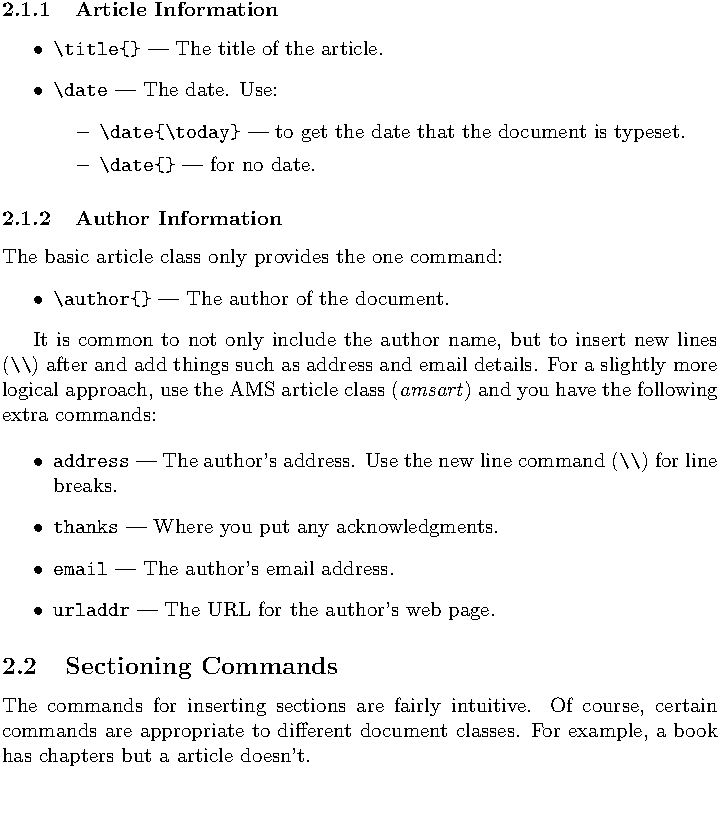
\includegraphics[width=.5\textwidth]{env5}}
% \end{center}
没什么新鲜东西,就不看效果了。下面抓紧说说怎么画表格。

\subsection{制作表格}

在这一小节,我们来尝试一下表格的输入。先起一个新“环境”,center,自然是“居中”的意思 :

\begin{enumerate}
\item[] \Cc\Ce center \Cj
\end{enumerate}

得到:

\begin{codeblock}[.9]
\begin{latexcode}
  % 此处略去数十行
 
  \subsection{Sectioning Commands}
  \label{sec:sectioning-commands}
  
  The commands for inserting sections are fairly intuitive.
  Of course, certain commands are appropriate to different
  document classes. For example, a book has chapters but a
  article doesn't.
  
  % A simple table. The center environment is first set up,
  % otherwise the table is left aligned.  The tabular
  % environment is what tells Latex that the data within is
  % data for the table.

  \begin{center}
    
  \end{center}
\end{latexcode}
\end{codeblock}

在center环境里面,我们添加一个 tabular(表格)环境:

\begin{enumerate}
\item[] \Cc\Ce{} tabular \Cj
\end{enumerate}

这时你会看到这样的提示:

\begin{enumerate}
\item[] \texttt{(Optional) Position:}
\end{enumerate}

Optional是可有可无的意思,也就是说,你如果在意表格的位置(Position),那么就提供位置信息;
如果不在意,那么就不用管它。现在我们连「位置」意味着什么都不清楚,自然就不必管它了。直接 \Cj{},又看到提示了:

\begin{enumerate}
\item[] \texttt{Format:}
\end{enumerate}

这是问你,表格的格式,比如该有几列?每列之间要不要有竖线分割?等等。我的答案是这样:

\begin{enumerate}
\item[] \texttt{|l|l|}
\end{enumerate}

也就是:竖线(|),小写L(l),竖线(|),小写L(l),竖线(|)。小写L代表 left,也就是“左对齐”的
意思。那么,你应该恍然大悟了,不就是……竖线-左对齐-竖线-左对齐-竖线嘛。那么,举一反三,除了
小写L,我们还会见到r(右对齐)和c(居中)。现在 \Cj{},得到如下结果:

\begin{codeblock}[.9]
\begin{latexcode}
  % 此处略去数十行
 
  \subsection{Sectioning Commands}
  \label{sec:sectioning-commands}
  
  The commands for inserting sections are fairly intuitive.
  Of course, certain commands are appropriate to different
  document classes. For example, a book has chapters but a
  article doesn't.
  
  % A simple table. The center environment is first set up,
  % otherwise the table is left aligned.  The tabular
  % environment is what tells Latex that the data within is
  % data for the table.

  \begin{center}
    \begin{tabular}{|l|l|}
      &
    \end{tabular}
  \end{center}
\end{latexcode}
\end{codeblock}

现在我们开始画表格,先画一条横线:

\begin{enumerate}
\item[] \verb'\hline' \Cj
\end{enumerate}

所谓 \verb'\hline' ,顾名思义,就是 horizontal line。画完横线,开始第一行,

\begin{enumerate}
\item[] \verb'Command & Level \\ \hline' \Cj
\end{enumerate}

那个 \verb'&' 就是两列之间的分隔符,``\verb'\\'''我们见过,表示强制换行。照猫画虎,把所有的
行都加上,得到如下结果:

\begin{codeblock}[.9]
\begin{latexcode}
  % 此处略去数十行
 
  \begin{center}
    \begin{tabular}{ll}
      \hline 
      Command & Level \\ \hline
      \verb|\part{}| & -1 \\
      \verb|\chapter{}| & 0 \\
      \verb|\section{}| & 1 \\
      \verb|\subsection{}| & 2 \\
      \verb|\subsubsection{}| & 3 \\
      \verb|\paragraph{}| & 4 \\
      \verb|\subparagraph{}| & 5 \\
      \hline
    \end{tabular}
  \end{center}
\end{latexcode}
\end{codeblock}

\begin{table}
  \begin{singlespace}
    \centering\caption{章节层次}\label{tab:level}
    \begin{tabular}{ll}\hline
      Command & Level \\ \hline
      \verb|\part{}| & -1 \\
      \verb|\chapter{}| & 0 \\
      \verb|\section{}| & 1 \\
      \verb|\subsection{}| & 2 \\
      \verb|\subsubsection{}| & 3 \\
      \verb|\paragraph{}| & 4 \\
      \verb|\subparagraph{}| & 5 \\ \hline
    \end{tabular}
  \end{singlespace}
\end{table}

这张表格的效果如表\ref{tab:level}所示。好了,表格画完了。再添加点文字:

\begin{codeblock}[.9]
\begin{latexcode}
  % 此处略去数十行 
  \begin{center}
    \begin{tabular}{ll}
      \hline 
      Command & Level \\ \hline
      \verb|\part{}| & -1 \\
      \verb|\chapter{}| & 0 \\
      \verb|\section{}| & 1 \\
      \verb|\subsection{}| & 2 \\
      \verb|\subsubsection{}| & 3 \\
      \verb|\paragraph{}| & 4 \\
      \verb|\subparagraph{}| & 5 \\
      \hline
    \end{tabular}
  \end{center}

  Numbering of the sections is performed automatically by
  \LaTeX{}, so don't bother adding them explicitly, just
  insert the heading you want between the curly braces. If
  you don't want sections number, then add an asterisk (*)
  after the section command, but before the first curly
  brace, e.g., \verb|section*{A Title Without Numbers}|.
\end{latexcode}
\end{codeblock}

现在编译一下,看看效果:

\begin{center}
  \fbox{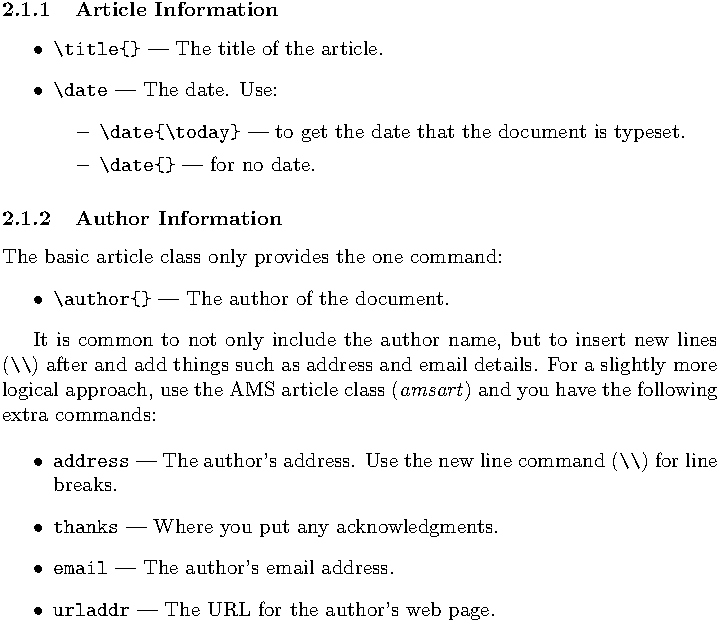
\includegraphics[width=.4\textwidth]{env6-crop-1}}
  \fbox{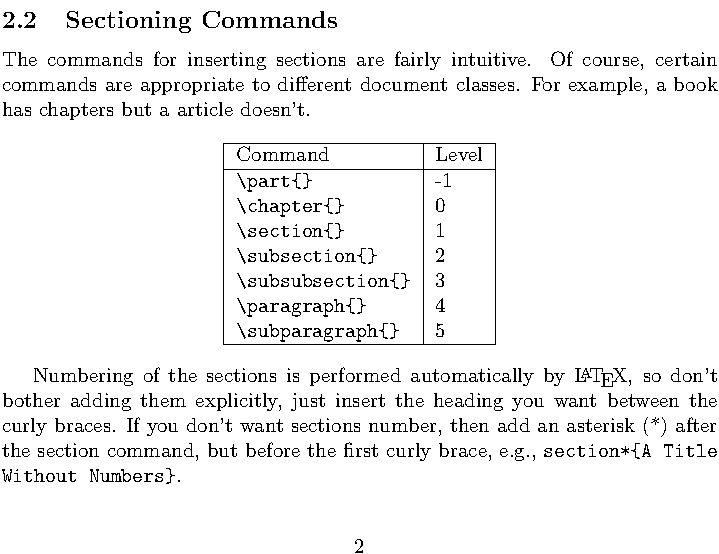
\includegraphics[width=.4\textwidth]{env6-crop-2}}
\end{center}

\subsection{引用参考文献}
\label{sec:ref}

处理参考文献,在\LaTeX{}中有两个选择:
\begin{itemize}
\item 传统的\bibtex{};
\item 时尚的\biblatex{}。
\end{itemize}
至于说两者的区别,粗略地说,\biblatex{}就是\bibtex{}的改进版。所以,下面我们只简要介绍一下
基于\biblatex{}的参考文献排版。

\subsubsection{第一步:准备好一个 \texttt{.bib} 文件}
Bib就是 Bibliography(参考文献)一词的前三个字母。顾名思义,在这个\texttt{.bib}文件里放的
都是你要用到的参考文献。我们这个小教程所用到的\texttt{tutorial.bib}文件就是个典型的例子。
节约篇幅起见,我们只列出该文件中的前三条记录如下:

\begin{longlisting}
\begin{bibtexcode}
@Misc{biblatex,
  author = {Philipp Lehman and Philip Kime and Audrey Boruvka and Joseph Wright},
  title = {The biblatex Package},
  month = 11,
  year = 2016}

@misc{ simple,
  author = "Andrew Roberts",
  title = "A simple article to illustrate document structure",
  year = 2003,
  url = "https://en.wikibooks.org/wiki/LaTeX/simple.tex",
}
@Book{Goossens94a,
  Title = {The LaTeX Companion},
  Author = {Michel Goossens and Frank Mittelbach and Alexander Samarin},
  Publisher = {Addison-Wesley},
  Year = 1994,
  Edition = {2nd revised},
}
\end{bibtexcode}
\end{longlisting}

怎么样,不难理解吧?照猫画虎地写出你自己的\texttt{.bib}文件应该不是件太困难的事情。

\subsubsection{第二步:引用参考文献}

准备好了你自己的\texttt{.bib}之后,剩下的事情就很简单了。简而言之,只要在你的\texttt{.tex}
文件里做三件事情……

首先,在\texttt{.tex}文件的\texttt{preamble}部分(也就是\verb|\begin{document}|之前)加上如
  下一行(假设你的\texttt{.bib}文件名字是\texttt{myref.bib}):
\begin{codeblock}
  \begin{latexcode}
    \addbibresource{myref.bib}
  \end{latexcode}
\end{codeblock}

然后,在\texttt{.tex}文件中的适当地方,你要引用到你的参考文献(也就是\texttt{.bib}文件中
的相应条目)。举个例子:

\rule{.9\textwidth}{.4pt}\\[-5ex]
\singlespacing
\begin{minipage}[t]{.45\linewidth}
  \textbf{\latex:}
  \begin{minted}[fontsize=\small,
linenos=false,%numbersep=10pt,
frame=none,%framesep=3pt,rulecolor=\color{lightgray},
xleftmargin=0cm,%xrightmargin=4cm,
%gobble=4
]{latex}
在\biblatex{}手册中,作者说到,
\biblatex{}是对\latex{}的参考文献
处理模块的彻底改进\cite{biblatex}。
\end{minted}
\end{minipage}
\hfill\vline\hfill
\begin{minipage}[t]{.45\linewidth}
  \textbf{PDF:}\\[1.5ex]  
  在\biblatex{}手册中,作者说到,\biblatex{}是对\latex{}的参考文献处理模块的彻底改
  进\cite{biblatex}。
\end{minipage}
\begin{center}
\rule{0.9\textwidth}{.1pt}
\end{center}
\doublespacing

上例中的\verb|\cite{biblatex}|就是要引用\texttt{myref.bib}中的第一条记录。在编译后输出的
PDF文件中我们会看到“\cite{biblatex}”。至于为什么是“6”而不是“1”或者其它什么数字,这取
决于生成参考文献时的排序选择,我们暂时不用关心它。

在\texttt{.tex}文件中要做的第三件事情是,在参考文献应该出现的地方加上如下一行:

\begin{codeblock}
\begin{latexcode}
\printbibliography{}
\end{latexcode}
\end{codeblock}

通常,“参考文献”应该作为一个章节出现在你的文章(或论文)的末尾。

\subsubsection{第三步:编译}

在上面的两步中,我们分别准备好了\texttt{.bib}和\texttt{.tex}文件,现在调用\texttt{latexmk}来编
译一下就行了。

前面我们都是用\texttt{xelatex}编译\texttt{.tex}文件,从来没提过\texttt{latexmk}。其实,不
用\texttt{latexmk}当然也可以完成文件的编译,具体步骤就是:
\vspace{-3ex}
\begin{singlespace}
  \begin{enumerate}
  \item \texttt{xelatex texfilename}
  \item \texttt{biber texfilename}
  \item \texttt{xelatex texfilename}
  \item 也许还要再执行一次上一行命令
  \end{enumerate}
\end{singlespace}
上面的第二步(调用\texttt{biber})就是用来处理参考文献的。如果觉得敲这三四个命令麻烦,那我
们就改用\texttt{latexmk}算了,唯一的前提条件是准备好一个小配置文件\texttt{.latexmkrc},内容
如下:
\begin{codeblock}[.9]
\begin{shellcode}
$pdf_mode = 1; $postscript_mode = $dvi_mode = 0;
$pdflatex = 'xelatex -interaction=nonstopmode -8bit --shell-escape %O %S';

$bibtex_use = 1;
$biber = 'biber --debug %O %S';
\end{shellcode}
\end{codeblock}

把这个小文件放到你自己的\verb|$HOME|目录下就行了。然后,只要:

\begin{codeblock}[.9]
  \begin{shellcode}
    latexmk texfilename
  \end{shellcode}
\end{codeblock}
不出错的话,一个带参考文献的PDF文件就诞生了。参考文献的样式就和本文的第\pageref{p:ref}页
差不多。

\section{小结}

本章我们利用Andrew Roberts的\texttt{simple.tex}了解了一下\LaTeX{}中最常用的命令和环境,同时
也熟悉了一下Emacs的基本键盘操作,在此做个小结。

\LaTeX{}最常用到的命令和环境:

\begin{center}
  \begin{tabular}{|l|l|l|}
    \hline%
    \verb'\title{}'&\verb'\author{}'&\verb'\date{}'\\\hline
    \verb'\section{}'&\verb'\subsection{}'&\verb'\subsubsection'\\\hline
    \texttt{itemize}&\texttt{center}&\texttt{tabular}\\\hline
  \end{tabular}
\end{center}

最基本的Emacs快捷键:\label{p:keys}%(大多以\Cx{}开头)
\vskip 1ex
\begin{onehalfspace}
  \begin{itemize}
  \item[] \textbf{文件操作:}
    \begin{tabular}{rl}\hline
      打开文件:&\Cx\Cf{}\\
      存盘:&\Cx\Cs{}\\
      关掉文件:&\Cx{\kbd k}\\
    \end{tabular}
  \item[] \textbf{编辑操作:}
    \begin{tabular}{rlrl}\hline
      终止命令:&\Cg{}&设置标记:&{\kbd }+{\kbd }\\
      换行缩进:&\Cj{}&缩进:&\Ci{}\\
      取消操作:&\Cslash{}&删除字符:&\Cd{}\\
      剪切:&\Ck{}&粘贴:&\Cy{}\\\hline
    \end{tabular}
  \item[] \textbf{移动光标:}
    \begin{tabular}{rlrl}
      向前:&\Cf{}&向后:&\Cb{}\\
      行首:&\Ca{}&行尾:&\Ce{}\\
      下一行:&\Cn{}&\hspace{1em}上一行:&\Cp{}\\
      \hspace{1em}下一页:&\Cv{}&上一页:&\Mv{}\\
    \end{tabular}
  \item[] \textbf{窗口操作:}
    \begin{tabular}{rlrl}\hline
      横分:&\Cx{}{\kbd 2}&纵分:&\Cx{}{\kbd 3}\\
      \hspace{1em}保留我:&\Cx{}{\kbd 1}&关掉我:&\Cx{}{\kbd 0}\\
      切换:&\Cx{}{\kbd o}&&\\\hline
    \end{tabular}
  \item[] \textbf{寻求帮助:}
    \begin{tabular}{rlrl}
      教程:&\Ch{}{\kbd t}&info:&\Ch{}{\kbd i}\\
      \hspace{1em}快捷键:&\Ch{}{\kbd k}&\hspace{1em}函数:&\Ch{}{\kbd f}\\
      变量:&\Ch{}{\kbd v}&&\\\hline
    \end{tabular}
  \end{itemize}
\end{onehalfspace}
\vskip 2ex
最基本的\auctex{}快捷键(大多以\Cc{}开头)

\begin{onehalfspace}
  \begin{center}
    \begin{tabular}{rl|rl}\hline
      环境:&\Cc\Ce{}&章节:&\Cc\Cs{}\\
      命令:&\Cc\Cm{}&换行:&\MEnter{}\\
      编译:&\Cc\Cc{}&查看:&\Cc\Cv\\\hline
    \end{tabular}
  \end{center}
\end{onehalfspace}

有了这些入门基础,我们已经可以应付要求不甚严格的文章排版了。但如果想排版出高质量的毕业论
文,hmm...,同志仍需努力。

在后续章节里,我们将简要介绍如下一些内容:

\begin{enumerate}
\item 如何插入图片
\item 如何写数学公式
\item 如何插入程序代码
\item 如何写中文
\item 如何使用毕业论文模版
% \item 如何做幻灯片
% \item Emacs org-mode
\end{enumerate}

%%% Local Variables:
%%% mode: latex
%%% TeX-master: "../tutorial"
%%% End:
